\documentclass[tikz, margin=5mm]{standalone}
\usepackage[sfdefault,light]{roboto}
\usetikzlibrary{
	arrows,
	arrows.meta,
	chains,
	positioning,
	shapes,
	shapes.multipart,
	mindmap,
	fit,
	calc,
	intersections,
	backgrounds,
	scopes,
	matrix,
	shadows,
}
\definecolor{MyGreen}{HTML}{41B3A3}
\tikzset{every picture/.style={/utils/exec={\sffamily}}}
\begin{document}
    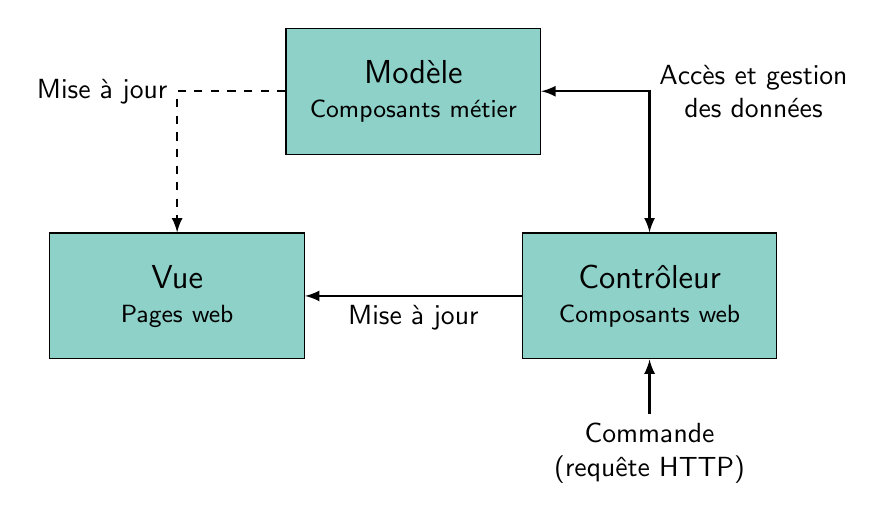
\begin{tikzpicture} [
            every node/.style={align=center,rectangle},
            comp/.style={draw,fill=MyGreen!60,minimum width=30mm,minimum height=16mm,text width=30mm,execute at begin node=\setlength{\baselineskip}{0.8em}}
        ]
        \node at (3,2) [comp] (model) {
            \large Modèle \\ [0.8ex]
            \small Composants métier
        };
        
        \node at (0,-.6) [comp] (view) {
            \large Vue \\ [0.8ex]
            \small Pages web
        };		
        
        \node at (6,-.6) [comp] (controller) {
            \large Contrôleur \\ [0.8ex]
            \small Composants web
        };
        
        \node at (6,-2.6) (input) {Commande \\ (requête HTTP)};
        
        \path[latex-latex,draw,thick] (controller.north) |- coordinate[midway] (cm) (model.east);
        \node[right] at (cm) {Accès et gestion \\ des données};
        
        \path[-latex,draw,dashed,thick] (model.west) -| coordinate[midway] (mv) (view.north);
        \node [left] at (mv) {Mise à jour};
        
        \path[-latex,draw,thick] (controller.west) -- coordinate[midway] (cv1) (view.east);
        \node [below] at (cv1) {Mise à jour};
        \path[-latex,draw,thick] (input.north) -- (controller.south);
    \end{tikzpicture}
\end{document}